\chapter[Dirichlet Beta and the Gaussian Field]{The Dirichlet Beta Function and the Gaussian Field}\label{ch:beta}

The unitary automorphic representations of $\mathrm{GL}(1)$ over $\mathbb Q$ are, up to twists by $\lvert\cdot\rvert^{it}$, the primitive Dirichlet characters, and one of the simplest nontrivial ones is the character $\chi_{-4}$ of the Gaussian field $K=\mathbb Q(i)$: $\chi_{-4}(n)=0$ for even $n$, $\chi_{-4}(n)=1$ for $n\equiv1$ and $\chi_{-4}(n)=-1$ for $n\equiv3\pmod 4$. Its $L$ function is the Dirichlet beta function
\begin{equation}\label{beta:eq:beta}
\beta(s)=\sum_{n\ge 0}\frac{(-1)^n}{(2n+1)^s}=\sum_{n\ge1}\frac{\chi_{-4}(n)}{n^s}
=\prod_{p}\bigl(1-\chi_{-4}(p)p^{-s}\bigr)^{-1},\qquad \operatorname{Re} s>1,
\end{equation}
with $\beta(1)=\pi/4$ and $\beta(2)=0.9159656$, Catalan's constant. Since $\chi_{-4}$ is real, odd and primitive with root number one, the completed function
\begin{equation}\label{beta:eq:Lambda}
\Lambda(s)=\Bigl(\frac{4}{\pi}\Bigr)^{s/2}\Gamma\Bigl(\frac{s+1}{2}\Bigr)\beta(s)
\end{equation}
is entire of order one with $\Lambda(s)=\Lambda(1-s)$. The generalized Riemann hypothesis (GRH) for $\beta$ asserts that every zero of $\Lambda$ lies on $\operatorname{Re} s=\tfrac12$.

This chapter works out for $\beta$ the Thorin framework of Chapters~\ref{ch:10b} and \ref{ch:10d} \cite{polson2017,polson2018vdp}. For real primitive characters the closed form of the Thorin density, the GGC property to the right of the critical strip and the equivalence of GRH with the GGC property at every basepoint $\alpha>\frac12$ are Theorem~30 and Remark~32 of \cite{polson2018vdp}, and in this book they are the case of $\chi_{-4}$ of Theorem~\ref{thm:10dshift}; what $\beta$ adds is an explicit positive kernel, a signed L\'evy measure, and the question of what the signs of that measure can prove. The framework has three parts: a L\'evy form of the completed function to the right of the critical strip; the $2\sin^2$ lemma of Chapter~\ref{ch:10d} (Lemma~\ref{lem:10dsin2}, from \cite{polson2018vdp}), which turns the L\'evy measure of the primal function into the Thorin measure of its reciprocal; and Thorin's condition, that $\Lambda(\tfrac12)/\Lambda(\tfrac12+\sqrt v)$ is the Laplace transform of a generalized gamma convolution (GGC, Definition~\ref{def:ch10ggc}), whose analyticity in the cut plane excludes zeros off the critical line (Theorem~\ref{thm:10bmain}).

Three features make $\beta$ the natural first case beyond $\zeta$. Its Mellin kernel is the weight $3/2$ theta series $\eta^3$, positive by the product formula. Its prime atoms carry the weights $\chi_{-4}(n)\Lambda(n)$, negative at $3,7,11,19,\dots$, so Thorin positivity is no longer termwise but arithmetic. Finally $\zeta_K=\zeta\cdot\beta$: the trivial character of $\mathrm{GL}(1)$ over $K$ induces to the isobaric representation $1\boxplus\chi_{-4}$ of $\mathrm{GL}(2)$ over $\mathbb Q$, and Thorin densities respect this decomposition.

Sections~\ref{beta:sec:primal} to \ref{beta:sec:lemma} construct the primal law, the L\'evy form and the closed form $T_\alpha(y)=\operatorname{Re}(\Lambda'/\Lambda)(\alpha+i\sqrt y)/(2\pi\sqrt y)$ of the Thorin density. Sections~\ref{beta:sec:uncond} and \ref{beta:sec:grh} recall the GGC property for $\alpha\ge1$ and the equivalence of GRH with the GGC property for all $\alpha>\tfrac12$. Section~\ref{beta:sec:gauss} treats the Gaussian field and the limits of termwise bounds; Section~\ref{beta:sec:axis} shows that positivity is free on the real axis, can fail only in short windows, and that GRH is equivalent to the density on each line $\tfrac12<\operatorname{Re} s\le1$ being smallest on the real axis; Section~\ref{beta:sec:argument} identifies the Thorin measure with the argument of $\Lambda$. Sections~\ref{beta:sec:centre} and \ref{beta:sec:eta} treat the centre and the pair $(\eta,\chi_{12})$.


\section{The completed beta function and its primal law}\label{beta:sec:primal}

\subsection{The eta cube kernel}
Jacobi's identity gives, with $q=e^{2\pi i\tau}$,
\begin{equation}\label{beta:eq:jacobi}
\eta(\tau)^3=q^{1/8}\prod_{m\ge1}(1-q^m)^3=\sum_{n\ge0}(-1)^n(2n+1)q^{(2n+1)^2/8}.
\end{equation}
At $\tau=ix$ this is the theta series of $\chi_{-4}$,
\begin{equation}\label{beta:eq:theta}
\vartheta_\beta(x):=\eta(ix)^3=\sum_{n\ge1}\chi_{-4}(n)\,n\,e^{-\pi n^2x/4},
\end{equation}
and $\eta(i/x)=\sqrt x\,\eta(ix)$ gives $\vartheta_\beta(1/x)=x^{3/2}\vartheta_\beta(x)$.

\begin{proposition}[Mellin form; classical]\label{beta:prop:mellin}
For all $s\in\C$,
\begin{equation}\label{beta:eq:mellin}
\Lambda(s)=\frac{\sqrt\pi}{2}\int_0^\infty x^{(s-1)/2}\,\eta(ix)^3\,dx .
\end{equation}
\end{proposition}

\begin{proof}
For $\operatorname{Re} s>1$ integrate \eqref{beta:eq:theta} term by term, using
\[
\int_0^\infty x^{(s+1)/2-1}e^{-\pi n^2x/4}\,dx=\Gamma\Bigl(\frac{s+1}{2}\Bigr)\Bigl(\frac{4}{\pi n^2}\Bigr)^{(s+1)/2}
\]
and $\sum_n\chi_{-4}(n)\,n^{-s}=\beta(s)$; the result is $(4/\pi)^{(s+1)/2}\Gamma(\tfrac{s+1}{2})\beta(s)$, which equals $(2/\sqrt\pi)\Lambda(s)$. Since $\vartheta_\beta$ decays like $e^{-\pi x/4}$ at infinity and like $x^{-3/2}e^{-\pi/(4x)}$ at zero, the integral is entire.
\end{proof}

\begin{proposition}[Primal kernel]\label{beta:prop:kernel}
The function $\Phi_\beta(u)=e^{3u/2}\,\eta(ie^{2u})^3$ is even, strictly positive, and decays like $\exp(\tfrac32|u|-\tfrac\pi4e^{2|u|})$. For all $w\in\C$,
\begin{equation}\label{beta:eq:kernel}
\Lambda\bigl(\tfrac12+w\bigr)=\sqrt\pi\int_{-\infty}^{\infty}e^{wu}\Phi_\beta(u)\,du
=2\sqrt\pi\int_0^\infty\cosh(wu)\,\Phi_\beta(u)\,du .
\end{equation}
\end{proposition}

\begin{proof}
Evenness is the transformation law, and positivity is the product in \eqref{beta:eq:jacobi}, every factor $1-q^m$ being positive for $q=e^{-2\pi x}\in(0,1)$. The identity is \eqref{beta:eq:mellin} after $x=e^{2u}$.
\end{proof}

This is the theta series proof of the functional equation for odd characters \cite{iwanieckowalski2004}; the eta cube form is in \cite[Section~8.1]{polson2018vdp}, and the theta identity is recalled in Chapter~\ref{ch:11}. Up to normalisation, $\Phi_\beta$ is the P\'olya kernel of Lemma~\ref{lem:10bkernel} for $\Xi^{\mathrm{sd}}$, here $\Lambda(\tfrac12+z)$ up to a constant factor, and it is positive for the reason given after that lemma for eta products, whereas the positivity of the Riemann P\'olya kernel takes work; and unlike $\xi$, $\Lambda$ has no polar factor. The normalised kernel $\Phi_\beta/\int\Phi_\beta$ is the density of a symmetric random variable $X_\beta$, the P\'olya variable of $\Xi^{\mathrm{sd}}$, which we call the \emph{primal law}, with
\begin{equation}\label{beta:eq:primal}
\E\bigl[e^{wX_\beta}\bigr]=\frac{\Lambda(\tfrac12+w)}{\Lambda(\tfrac12)},\qquad
\E\bigl[e^{itX_\beta}\bigr]=\frac{\Lambda(\tfrac12+it)}{\Lambda(\tfrac12)} .
\end{equation}
Numerically $\Lambda(\tfrac12)=0.86913481$, $\beta(\tfrac12)=0.66769146$ and $\Phi_\beta(0)=0.45338383$.

\subsection{Zeros and the tilt}

\begin{lemma}[No real zeros]\label{beta:lem:real}
$\beta(\sigma)\ge1-3^{-\sigma}>0$ for real $\sigma>0$. Hence $\Lambda$ has no zeros in $(0,1)$.
\end{lemma}

\begin{proof}
For $\sigma>0$ the series \eqref{beta:eq:beta} converges, alternates and has strictly decreasing terms.
\end{proof}

The zeros $\rho$ of $\Lambda$ are symmetric under $\rho\mapsto1-\rho$ and $\rho\mapsto\bar\rho$, and every zero satisfies $0<\operatorname{Re}\rho<1$ (the Euler product excludes $\operatorname{Re} s>1$, and the nonvanishing of $\beta$ on $\operatorname{Re} s=1$ with the functional equation excludes the edges). Writing $\rho=\tfrac12+i\theta$ (by Lemma~\ref{beta:lem:real} no $\theta$ is purely imaginary, so the condition $\operatorname{Re}\theta>0$ picks one of each pair $\pm\theta$), the functional equation gives $\Lambda'(\tfrac12)=0$ and kills the exponential factor of the Hadamard product, so
\begin{equation}\label{beta:eq:hadamard}
\frac{\Lambda(\tfrac12+w)}{\Lambda(\tfrac12)}=\prod_{\operatorname{Re}\theta>0}\Bigl(1+\frac{w^2}{\theta^2}\Bigr),
\qquad
\operatorname{Re}\frac{\Lambda'}{\Lambda}(s)=\sum_{\rho}\frac{\operatorname{Re} s-\operatorname{Re}\rho}{|s-\rho|^2},
\end{equation}
the sum converging absolutely since $\sum|\rho|^{-2}<\infty$. Under GRH every $\theta$ is a real ordinate $\gamma$ and $\Lambda(\tfrac12)/\Lambda(\tfrac12+w)=\prod_{\gamma>0}\gamma^2/(\gamma^2+w^2)$, the product \eqref{eq:10batoms} of Chapter~\ref{ch:10b} for $\Xi^{\mathrm{sd}}$. The first ordinates $\gamma$ are $6.02094890$, $10.24377030$, $12.98809801$, $16.34260710$ and $18.29199320$. We write
\begin{equation}\label{beta:eq:calpha}
c_\alpha:=\frac{\Lambda'}{\Lambda}(\alpha)=\tfrac12\log\frac4\pi+\tfrac12\psi\Bigl(\frac{\alpha+1}{2}\Bigr)+\frac{\beta'}{\beta}(\alpha)
\end{equation}
and $V:=(\log\Lambda)''(\tfrac12)=\mathrm{Var}(X_\beta)=0.156030$, twice the sum $S_1=0.078015$ of Table~\ref{tab:10bcatalogue}. By \eqref{beta:eq:hadamard}, $c_\alpha>0$ for $\alpha\ge1$, and $c_{1/2}=0$.


\section{The L\'evy form for \texorpdfstring{$\alpha>1$}{alpha > 1}}\label{beta:sec:levy}

\begin{theorem}[L\'evy form; as in Section~\ref{sec:10daway}]\label{beta:thm:levy}
For $\alpha>1$ and $\operatorname{Re} s\ge0$,
\begin{equation}\label{beta:eq:levy}
\log\frac{\Lambda(\alpha+s)}{\Lambda(\alpha)}-c_\alpha s=\int_0^\infty\bigl(e^{-sx}-1+sx\bigr)e^{-\alpha x}\,\frac{\mu_\beta(dx)}{x},
\end{equation}
with the signed measure
\begin{equation}\label{beta:eq:mubeta}
\mu_\beta(dx)=\frac{dx}{2\sinh x}+\sum_{n\ge2}\chi_{-4}(n)\,\Lambda(n)\,\delta_{\log n}(dx).
\end{equation}
\end{theorem}

\begin{proof}
The factor $(4/\pi)^{s/2}$ is absorbed by the tilt. For $\operatorname{Re} z>0$,
\[
\log\frac{\Gamma(z+v)}{\Gamma(z)}-v\psi(z)=\int_0^\infty\bigl(e^{-vx}-1+vx\bigr)\frac{e^{-zx}}{x(1-e^{-x})}\,dx,
\]
since both sides and their first derivatives vanish at $v=0$ and both have second derivative $\psi'(z+v)$. Taking $z=\tfrac{\alpha+1}{2}$, $v=\tfrac s2$ and $x\mapsto2x$ turns the kernel into $e^{-\alpha x}/(2x\sinh x)$. For the Dirichlet series, on $\operatorname{Re} s>1$ the function $\log\beta(s)$ is $\sum_{n\ge2}\chi_{-4}(n)\Lambda(n)(\log n)^{-1}n^{-s}$, which gives the atoms. Absolute convergence follows from $|e^{-sx}-1+sx|\le\min(2+|s|x,\tfrac12|s|^2x^2)$.
\end{proof}

With the prime sum truncated at $n\le2\times10^5$ the two sides of \eqref{beta:eq:levy} agree to seven digits at $(\alpha,s)=(2,2)$ and to twelve at $(3,2)$, where both equal $0.232881325700$.

\begin{remark}[Comparison with $\xi$]\label{beta:rem:xi}
For $\xi(s)=\tfrac12s(s-1)\pi^{-s/2}\Gamma(\tfrac s2)\zeta(s)$ the same computation gives the measure $-e^x\,dx+dx/(e^{2x}-1)+\sum_{n\ge2}\Lambda(n)\delta_{\log n}$. The polar factor $\alpha-1+s$ is log concave in $s$, so it enters with a negative sign (Section~\ref{sec:10daway}). For $\beta$ there is no polar term, the archimedean density is $1/(2\sinh x)$ (an odd character shifts the gamma argument by one half), and the prime part is the difference of two positive measures, carried by the prime powers $n\equiv1$ and $n\equiv3\pmod4$ respectively.
\end{remark}


\section{The \texorpdfstring{$2\sin^2$}{2 sin squared} lemma and the Thorin density}\label{beta:sec:lemma}

Lemma~\ref{lem:10dsin2} transports a positive L\'evy measure. The transport is linear in the measure, and it holds for a signed measure once the positivity conclusion is dropped; we state it in the Laplace variable $v=s^2$ and prove it by Fourier inversion, which also gives \eqref{beta:eq:logformula}.

\begin{lemma}[$2\sin^2$ lemma, signed form; after Lemma~\ref{lem:10dsin2}]\label{beta:lem:2sin2}
Let $f$ be analytic and nonvanishing near $[\alpha,\infty)$, let $c=f'(\alpha)/f(\alpha)$, and suppose that for $s\ge0$
\[
\log\frac{f(\alpha+s)}{f(\alpha)}-cs=\int_0^\infty\bigl(e^{-sx}-1+sx\bigr)\,m(dx)
\]
for a signed measure $m$ with $\int\min(x,x^2)\,|m|(dx)<\infty$. Put
\begin{equation}\label{beta:eq:Tdef}
T(y)=\frac{1}{2\pi\sqrt y}\Bigl[c+\int_0^\infty2\sin^2\Bigl(\frac{x\sqrt y}{2}\Bigr)x\,m(dx)\Bigr],\qquad y>0.
\end{equation}
Then for every $v>0$,
\begin{equation}\label{beta:eq:thorinrep}
\frac{f(\alpha)}{f(\alpha+\sqrt v)}=\exp\Bigl(-\int_0^\infty\log\Bigl(1+\frac vy\Bigr)T(y)\,dy\Bigr).
\end{equation}
The map $m\mapsto T$ is linear and positivity preserving, and $c\ge0$ contributes the positive stable part $c/(2\pi\sqrt y)$.
\end{lemma}

\begin{proof}
With $y=t^2$, $T(y)\,dy=\pi^{-1}\bigl[c+\int x(1-\cos tx)\,m(dx)\bigr]dt$. The integrals
\[
\int_0^\infty\log\Bigl(1+\frac{v}{t^2}\Bigr)dt=\pi\sqrt v,\qquad
\int_0^\infty\log\Bigl(1+\frac{v}{t^2}\Bigr)\cos(xt)\,dt=\frac{\pi}{x}\bigl(1-e^{-x\sqrt v}\bigr),
\]
the second by parts from $\int_0^\infty\sin(xt)\,dt/(t(t^2+v))=\pi(1-e^{-x\sqrt v})/(2v)$, give
\begin{align*}
\int_0^\infty\log\Bigl(1+\frac vy\Bigr)T(y)\,dy
&=c\sqrt v+\int_0^\infty\bigl(e^{-x\sqrt v}-1+x\sqrt v\bigr)m(dx)\\
&=\log\frac{f(\alpha+\sqrt v)}{f(\alpha)} ,
\end{align*}
Fubini being justified by $|1-\cos tx|\le\min(2,t^2x^2/2)$.
\end{proof}

If $f$ is analytic on $\operatorname{Re} s\ge\alpha$, differentiating the L\'evy form at $s=it$ gives $\operatorname{Re}(f'/f)(\alpha+it)-c=\int x(1-\cos tx)\,m(dx)$, so the bracket in \eqref{beta:eq:Tdef} is $\operatorname{Re}(f'/f)(\alpha+i\sqrt y)$. For $f=\Lambda$ this is the main formula of the chapter.

\begin{theorem}[Thorin density of the reciprocal beta function; \cite{polson2018vdp}, Theorem~30]\label{beta:thm:thorin}
For $\alpha>1$ and $v>0$,
\begin{equation}\label{beta:eq:thorinbeta}
\frac{\Lambda(\alpha)}{\Lambda(\alpha+\sqrt v)}=\exp\Bigl(-\int_0^\infty\log\Bigl(1+\frac vy\Bigr)T_\alpha(y)\,dy\Bigr),
\end{equation}
where
\begin{align}
T_\alpha(y)&=\frac{1}{2\pi\sqrt y}\Bigl[c_\alpha+\int_0^\infty2\sin^2\Bigl(\frac{x\sqrt y}{2}\Bigr)e^{-\alpha x}\mu_\beta(dx)\Bigr]\label{beta:eq:Tsin}\\
&=\frac{c_\alpha+G_\alpha(\sqrt y)+P_\alpha(\sqrt y)}{2\pi\sqrt y}
=\frac{1}{2\pi\sqrt y}\,\operatorname{Re}\frac{\Lambda'}{\Lambda}\bigl(\alpha+i\sqrt y\bigr),\label{beta:eq:Tclosed}
\end{align}
with the archimedean and prime parts
\begin{align*}
G_\alpha(t)&=\tfrac12\Bigl[\operatorname{Re}\,\psi\Bigl(\frac{\alpha+1+it}{2}\Bigr)-\psi\Bigl(\frac{\alpha+1}{2}\Bigr)\Bigr]\ge0,\\
P_\alpha(t)&=\sum_{n\ge2}\chi_{-4}(n)\Lambda(n)\,n^{-\alpha}\bigl(1-\cos(t\log n)\bigr).
\end{align*}
Equivalently,
\begin{equation}\label{beta:eq:logformula}
\log\frac{\Lambda(\alpha+\sqrt v)}{\Lambda(\alpha)}=\frac1\pi\int_0^\infty\log\Bigl(1+\frac{v}{t^2}\Bigr)\,\operatorname{Re}\frac{\Lambda'}{\Lambda}(\alpha+it)\,dt .
\end{equation}
\end{theorem}

\begin{proof}
Apply Lemma~\ref{beta:lem:2sin2} to Theorem~\ref{beta:thm:levy}. The density satisfies $T_\alpha(y)\sim c_\alpha/(2\pi\sqrt y)$ as $y\to0$, and $T_\alpha(y)=O(\log y/\sqrt y)$ as $y\to\infty$ because $P_\alpha$ is bounded and $\operatorname{Re}\,\psi(\tfrac{\alpha+1+it}{2})\sim\log(t/2)$.
\end{proof}

In the notation of Theorem~\ref{thm:10dshift}, whose $\Xi_\pi$ is $\Lambda(\tfrac12+z)^2$ up to a constant factor, $2T_\alpha=V_{\alpha-1/2}$, and $T_\alpha(y)\,dy$ is the Thorin measure $\tau$ (Definition~\ref{def:ch10ggc}) of $\Lambda(\alpha)/\Lambda(\alpha+\sqrt v)$ when every zero of $\Lambda$ has real part less than $\alpha$ (for every $\alpha\ge1$ by part~(iii) of that theorem, and for every $\alpha>\frac12$ under GRH).

The sine squared form \eqref{beta:eq:Tsin}, with primes to $2\times10^5$, and the closed form \eqref{beta:eq:Tclosed} give the same values of $2\pi t\,T_\alpha(t^2)$, namely $0.2353511$, $0.7691193$ and $0.32628$ at $(\alpha,t)=(2,1),(2,7),(\tfrac32,4)$. Formula \eqref{beta:eq:logformula} at $(\alpha,v)=(2,1)$, by quadrature to $t=150$ plus the archimedean tail $v(\log(2T/\pi)+1)/(2\pi T)$ at $T=150$, gives $0.2977961$ against $\log\Lambda(3)/\Lambda(2)=0.2977947$; the residual comes from the oscillating prime part beyond $t=150$.


\section{What holds unconditionally}\label{beta:sec:uncond}

\begin{theorem}[GGC for $\alpha\ge1$; Theorem~\ref{thm:10dshift}(iii)]\label{beta:thm:uncond}
For every $\alpha\ge1$ there is a GGC random variable $H^\beta_\alpha\ge0$, with drift zero and Thorin density $T_\alpha>0$ given by \eqref{beta:eq:Tclosed}, such that
\[
\frac{\Lambda(\alpha)}{\Lambda(\alpha+\sqrt v)}=\E\bigl[e^{-vH^\beta_\alpha}\bigr],\qquad v>0.
\]
In particular $\tfrac{\sqrt\pi}{2}\big/\Lambda(1+\sqrt v)$ is a GGC Laplace transform.
\end{theorem}

\begin{proof}
Since every zero has $\operatorname{Re}\rho<1$, each term of \eqref{beta:eq:hadamard} is positive on $\operatorname{Re} s=\alpha\ge1$, so $T_\alpha>0$. By Theorem~\ref{thm:10dshift}(iii) with $a=\alpha-\frac12$, the square $(\Lambda(\alpha)/\Lambda(\alpha+\sqrt v))^2$ is the transform of a GGC with drift zero and Thorin density $V_{\alpha-1/2}=2T_\alpha$, so by Definition~\ref{def:ch10ggc} its square root is the transform of a GGC with drift zero and Thorin density $T_\alpha$. For $\alpha>1$ this is also Theorem~\ref{beta:thm:thorin}.
\end{proof}

The proof uses the zeros rather than the L\'evy measure. On the L\'evy side the sine squared integrand in \eqref{beta:eq:Tsin} is signed, and bounding the atoms by their absolute values proves positivity at every height only above a threshold $\alpha_c$. Write
\begin{align}
A_\alpha(t)&=\tfrac12\log\frac4\pi+\tfrac12\operatorname{Re}\,\psi\Bigl(\frac{\alpha+1+it}{2}\Bigr),\notag\\
S(\alpha)&=\sum_{n\text{ odd}}\Lambda(n)n^{-\alpha}=-\frac{\zeta'}{\zeta}(\alpha)-\frac{\log2}{2^\alpha-1},\label{beta:eq:AS}
\end{align}
so that $\operatorname{Re}\,\Lambda'/\Lambda(\alpha+it)=A_\alpha(t)+\operatorname{Re}\,\beta'/\beta(\alpha+it)$ and $|\beta'/\beta(\alpha+it)|\le S(\alpha)$ for $\alpha>1$.

\begin{proposition}[Termwise positivity]\label{beta:prop:crude}
$A_\alpha(t)$ increases in $t$, $A_\alpha(0)$ increases in $\alpha$, and $S(\alpha)$ decreases. Let $\alpha_c$ be the root of $A_\alpha(0)=S(\alpha)$, numerically $\alpha_c=2.28231064$. For $\alpha\ge\alpha_c$ the bound $A_\alpha(t)-S(\alpha)$ proves $T_\alpha(t^2)>0$ for all $t>0$; for $1<\alpha<\alpha_c$ it fails near $t=0$, although $T_\alpha>0$ by Theorem~\ref{beta:thm:uncond}.
\end{proposition}

\begin{proof}
Monotonicity in $t$ follows from $\operatorname{Re}\,\psi(x+iy)-\psi(x)=\sum_{k\ge0}y^2/\bigl((x+k)((x+k)^2+y^2)\bigr)$; $\psi$ increases on $(0,\infty)$, and $S$ is a Dirichlet series with positive coefficients.
\end{proof}

At $\alpha=\tfrac32$ (Figure~\ref{beta:fig:thorin}, right) the prime part $P_\alpha$ is negative over most of $[0,30]$, with minimum $-0.532$ near $t=19.9$, where $c_\alpha+G_\alpha=1.418$. For $\zeta$ the corresponding prime part is a positive sum.

\begin{figure}[t]
\centering
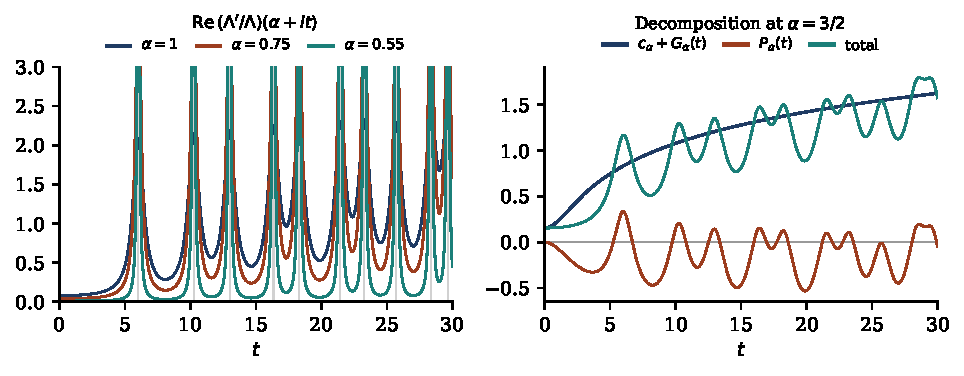
\includegraphics[width=\textwidth]{figs/beta_thorin.pdf}
\caption{Left: $\operatorname{Re}(\Lambda'/\Lambda)(\alpha+it)=2\pi t\,T_\alpha(t^2)$ for $\alpha=1,\,0.75,\,0.55$ and $0\le t\le30$, with the vertical axis cut at $3$; grey lines mark the ordinates of the zeros of $\beta$. As $\alpha\downarrow\frac12$ the density concentrates on the zeros. Right: at $\alpha=\frac32$, the archimedean part with the constant, $c_\alpha+G_\alpha$, the signed prime part $P_\alpha$, and their sum (labelled total).}
\label{beta:fig:thorin}
\end{figure}


\section{GRH as Thorin positivity}\label{beta:sec:grh}

\begin{theorem}[GRH as Thorin positivity; Theorem~\ref{thm:10dshift}(iv) and \cite{polson2018vdp}, Remark~32]\label{beta:thm:grh}
The following are equivalent.
\begin{enumerate}
\item[(i)] GRH for $\beta$.
\item[(ii)] For every $\alpha>\tfrac12$, $\Lambda(\alpha)/\Lambda(\alpha+\sqrt v)$ is the Laplace transform of a GGC.
\item[(iii)] $\operatorname{Re}\,(\Lambda'/\Lambda)(s)>0$ for $\operatorname{Re} s>\tfrac12$.
\end{enumerate}
In this case the Thorin measures $T_\alpha(y)\,dy$ converge vaguely on $(0,\infty)$, as $\alpha\downarrow\tfrac12$, to $\sum_{\gamma>0}\delta_{\gamma^2}$ counted with multiplicity, the Thorin measure of $\Lambda(\tfrac12)/\Lambda(\tfrac12+\sqrt v)$.
\end{theorem}

\begin{proof}
Up to a constant factor $\Lambda(\tfrac12+z)^2$ is the function $\Xi_\pi$ of Theorem~\ref{thm:10dshift}, and by Definition~\ref{def:ch10ggc} a GGC transform has GGC square and square root. So (i)$\Rightarrow$(ii) is part (i) of that theorem for every $a=\alpha-\frac12>0$, and (ii)$\Rightarrow$(i) is its part (ii), the cut plane argument of Lemma~\ref{lem:ch10nonvanish}, for every $a>0$. (i)$\Rightarrow$(iii) is \eqref{beta:eq:hadamard}. (iii)$\Rightarrow$(i): a zero $\rho$ of multiplicity $m$ with $\operatorname{Re}\rho>\tfrac12$ is a pole of $\Lambda'/\Lambda$ with residue $m$, so $\operatorname{Re}\,\Lambda'/\Lambda(s)=m\operatorname{Re}(s-\rho)^{-1}+O(1)$ takes negative values for $s$ near $\rho$ with $\operatorname{Re} s<\operatorname{Re}\rho$. The limit is part (iv) of the theorem: under (i), with $a=\alpha-\tfrac12$ and $y=t^2$, $T_\alpha(y)\,dy=\pi^{-1}\sum_\gamma a\,(a^2+(t-\gamma)^2)^{-1}dt$ is a sum of Poisson kernels, which converges to $\sum_{\gamma>0}\delta_\gamma(dt)$ on $t>0$.
\end{proof}

The equivalence of (i) and (iii) is the criterion of Hinkkanen \cite{hinkkanen1997} and Lagarias \cite{lagarias1999} for $\chi_{-4}$ (Lagarias's Theorem~1.1 is stated for any admissible set of zeros), and Theorem~\ref{thm:10dshift}(iv) is its Thorin form. The two conditions are one statement in two variables: the Thorin density at $y=t^2$ is $\operatorname{Re}\,\Lambda'/\Lambda$ at height $t$ divided by $2\pi t$. For $\xi$ more is known: the minimum of $\operatorname{Re}\,\xi'/\xi$ on the line $\operatorname{Re}s=\alpha$ is attained only at $t=0$ under RH for every $\alpha>\frac12$ (Lagarias's Theorem~1.3 and its proof in Section~3), and at $t=0$ unconditionally for every $\alpha\ge1$ (Garunk\v{s}tis \cite{garunkstis2002}). Numerically the same holds for $\beta$: over $t\in[0,50]$ the minimum of $\operatorname{Re}\,\Lambda'/\Lambda(\alpha+it)$ is $c_\alpha$, attained at $t=0$:

\begin{center}
\begin{tabular}{ccccc}
\toprule
$\alpha$ & $1$ & $0.75$ & $0.6$ & $0.55$\\
\midrule
$c_\alpha$ & $0.077784$ & $0.038978$ & $0.015601$ & $0.007801$\\
$c_\alpha/(\alpha-\frac12)$ & $0.1556$ & $0.1559$ & $0.1560$ & $0.1560$\\
\bottomrule
\end{tabular}
\end{center}

\noindent The margin at $t=0$ shrinks like $(\alpha-\tfrac12)V$, while near each ordinate the density grows like $(\alpha-\tfrac12)^{-1}$. Section~\ref{beta:sec:axis} shows (Theorem~\ref{beta:thm:minall}) that for $\frac12<\alpha\le3.15$ the real axis is the minimum, unconditionally, for $|t|\le H_0-1.21$, where $H_0$ is the height to which GRH for $\beta$ has been verified.



\section{The Gaussian field and termwise bounds}\label{beta:sec:gauss}

\subsection{Automorphic induction and Thorin densities}

Let $K=\mathbb Q(i)$, with $\zeta_K(s)=\sum_{\mathfrak a}N(\mathfrak a)^{-s}$ over the nonzero ideals of $\mathbb Z[i]$. A prime $p\equiv1\pmod 4$ splits into two Gaussian primes of norm $p$, a prime $p\equiv3\pmod4$ is inert with norm $p^2$, and $2$ ramifies; this splitting law is the identity $\zeta_K=\zeta\cdot\beta$, and by class field theory $\chi_{-4}$ is the quadratic character of $\mathrm{Gal}(K/\mathbb Q)$. In the Langlands picture the trivial character of $\mathrm{GL}(1)$ over $K$ induces to the isobaric representation $1\boxplus\chi_{-4}$ of $\mathrm{GL}(2)$ over $\mathbb Q$, whose standard $L$ function is $\zeta\beta$. The pairing of the atoms at $p\equiv1$ and $p\equiv3\pmod 4$ is exactly this splitting.

\begin{remark}[Isobaric sums]\label{beta:rem:isobaric}
The closed form \eqref{beta:eq:Tclosed} is linear in the logarithmic derivative, so if $\Lambda_\pi=\Lambda_{\pi_1}\Lambda_{\pi_2}$ for an isobaric sum $\pi=\pi_1\boxplus\pi_2$, then $T^\pi_\alpha=T^{\pi_1}_\alpha+T^{\pi_2}_\alpha$ on every vertical line and, on lines $\operatorname{Re}s=\alpha$ to the right of every zero of both functions (every $\alpha\ge1$, and every $\alpha>\frac12$ under GRH for both), the GGC variables of the reciprocals are independent summands. Positivity of the summands implies positivity of the sum but not conversely, which is why Thorin positivity for a component becomes a domination statement inside the sum.
\end{remark}

\subsection{Thorin domination}

Put $\xi_K(s)=\tfrac12s(s-1)\pi^{-s}\Gamma(s)\zeta_K(s)$.

\begin{proposition}[Factorisation]\label{beta:prop:factor}
$\Lambda(s)=2\sqrt\pi\,\xi_K(s)/\xi(s)$. For $\alpha>1$ the L\'evy measures satisfy $\mu_\beta=\mu_K-\mu_\xi$, where
\begin{align*}
\mu_K(dx)&=-e^x\,dx+\frac{dx}{e^x-1}+\sum_{n\ge2}\Lambda(n)\bigl(1+\chi_{-4}(n)\bigr)\delta_{\log n}(dx),\\
\mu_\xi(dx)&=-e^x\,dx+\frac{dx}{e^{2x}-1}+\sum_{n\ge2}\Lambda(n)\,\delta_{\log n}(dx).
\end{align*}
Apart from the common polar term, both measures are positive.
\end{proposition}

\begin{proof}
The duplication formula $\Gamma(s)=2^{s-1}\pi^{-1/2}\Gamma(\tfrac s2)\Gamma(\tfrac{s+1}2)$ gives
\[
\frac{\pi^{-s}\Gamma(s)}{\pi^{-s/2}\Gamma(\tfrac s2)}=\frac{1}{2\sqrt\pi}\Bigl(\frac4\pi\Bigr)^{s/2}\Gamma\Bigl(\frac{s+1}{2}\Bigr).
\]
The measures follow as in Theorem~\ref{beta:thm:levy} and Remark~\ref{beta:rem:xi}: $\tfrac12s(s-1)\Gamma(s)=(s-1)\Gamma(s+1)/2$ gives $-e^x\,dx$ and $1/(e^x-1)$, and $-\zeta_K'/\zeta_K$ has coefficients $\Lambda(n)(1+\chi_{-4}(n))\ge0$. The polar terms cancel and $1/(e^x-1)-1/(e^{2x}-1)=1/(2\sinh x)$.
\end{proof}

\begin{theorem}[Thorin domination; positivity and equivalence by Theorem~\ref{thm:10dshift}]\label{beta:thm:dom}
Let $T^K_\alpha$ and $T^\xi_\alpha$ be the Thorin densities given by \eqref{beta:eq:Tclosed} with $\xi_K$ and $\xi$ in place of $\Lambda$, that is, those of $\xi_K(\alpha)/\xi_K(\alpha+\sqrt v)$ and $\xi(\alpha)/\xi(\alpha+\sqrt v)$. Then $T^\beta_\alpha=T^K_\alpha-T^\xi_\alpha$. For $\alpha\ge1$ all three densities are positive and there are independent GGC variables with $H^K_\alpha\overset{d}{=}H^\xi_\alpha+H^\beta_\alpha$. GRH for $\beta$ holds if and only if $T^K_\alpha\ge T^\xi_\alpha$ for every $\alpha>\tfrac12$; if Thorin's condition holds for $\xi$, this says that $H^\xi_\alpha$ is a GGC factor of $H^K_\alpha$ for every $\alpha>\tfrac12$.
\end{theorem}

\begin{proof}
By Proposition~\ref{beta:prop:factor}, $\operatorname{Re}\,\Lambda'/\Lambda=\operatorname{Re}\,\xi_K'/\xi_K-\operatorname{Re}\,\xi'/\xi$ on every vertical line. Positivity for $\alpha\ge1$ (strict, since every term of the Hadamard sums is then positive, as in the proof of Theorem~\ref{beta:thm:uncond}) and the equivalence are parts (iii) and (iv) of Theorem~\ref{thm:10dshift} for $\zeta$, where $\Xi_\zeta(z)=\xi(\tfrac12+z)$, and for $\chi_{-4}$, where $\Xi_\pi(z)$ is $\Lambda(\tfrac12+z)^2$ up to a constant factor and has density $2T_\alpha$ (see also \cite[Theorem~30 and Remark~32]{polson2018vdp}).
\end{proof}

At $\alpha=\tfrac32$ and $t=0,2,5,10,20$:

\begin{center}
\begin{tabular}{cccccc}
\toprule
$t$ & $0$ & $2$ & $5$ & $10$ & $20$\\
\midrule
$\operatorname{Re}\,\xi_K'/\xi_K$ & $0.20035$ & $0.22524$ & $0.68519$ & $1.32766$ & $1.49863$\\
$\operatorname{Re}\,\xi'/\xi$ & $0.04614$ & $0.04704$ & $0.05267$ & $0.10289$ & $0.60611$\\
$\operatorname{Re}\,\Lambda'/\Lambda$ & $0.15422$ & $0.17820$ & $0.63252$ & $1.22477$ & $0.89252$\\
\bottomrule
\end{tabular}
\end{center}

\subsection{Kronecker sharpness}

The factorisation is the right language for pairing, but it cannot lower $\alpha_c$ on its own, because the termwise bound is sharp.

\begin{proposition}[Kronecker sharpness]\label{beta:prop:kron}
For $\alpha>1$ and every $T>0$,
\[
\inf_{t\ge T}\operatorname{Re}\frac{\beta'}{\beta}(\alpha+it)=-S(\alpha).
\]
Hence a bound on the prime part that uses only $|\chi_{-4}(p)|$ proves $T_\alpha(t^2)>0$ exactly for $t>t_0(\alpha)$, where $A_\alpha(t_0)=S(\alpha)$ (and $t_0=0$ for $\alpha\ge\alpha_c$), and $\log t_0(\alpha)=2/(\alpha-1)+O(1)$ as $\alpha\downarrow1$.
\end{proposition}

\begin{proof}
From the Euler product, $\operatorname{Re}\,\beta'/\beta(\alpha+it)=-\sum_p\log p\,\operatorname{Re}\,w_p/(1-w_p)$ with $w_p=\chi_{-4}(p)p^{-\alpha-it}$, and $\operatorname{Re}\,w/(1-w)\le r/(1-r)$ on $|w|=r<1$ with equality at $w=r$. As in the proof of Proposition~\ref{prop:ch09notcf}, the $\log p$ are linearly independent over $\mathbb Q$, so Kronecker's theorem gives $t\ge T$ with $\chi_{-4}(p)p^{-it}$ arbitrarily close to $1$ for all $p\le P$, and the tail over $p>P$ is small. The asymptotic uses $S(\alpha)=(\alpha-1)^{-1}+O(1)$ and $A_\alpha(t)=\tfrac12\log t+O(1)$.
\end{proof}

\begin{center}
\begin{tabular}{ccccccc}
\toprule
$\alpha$ & $2$ & $1.75$ & $1.5$ & $1.25$ & $1.1$ & $1.05$\\
\midrule
$S(\alpha)$ & $0.339$ & $0.580$ & $1.126$ & $2.964$ & $8.835$ & $18.78$\\
$t_0(\alpha)$ & $2.37$ & $4.72$ & $14.9$ & $589$ & $7.4\times10^7$ & $3.3\times10^{16}$\\
\bottomrule
\end{tabular}
\end{center}

\noindent For each $\alpha\in(1,\alpha_c)$ the elementary route thus reduces positivity to a finite computation with error control on $[0,t_0(\alpha)]$, but the range grows like $e^{2/(\alpha-1)}$. The route does not reach $\alpha=1$. There the GGC property itself follows from $\alpha>1$, since GGC laws are closed under weak limits; what needs the nonvanishing of $\beta$ on $\operatorname{Re}s=1$, that is the prime number theorem for primes modulo $4$, is that the Thorin measure at $\alpha=1$ is $T_1(y)\,dy$, with no atom at the square of the ordinate of a zero on that line (for $\xi$, \cite[Remark~21]{polson2018vdp}). The sizes of the atoms do not contain this information. Dirichlet's theorem for the modulus $4$ needs only $\beta(1)=\pi/4\ne0$.


\section{The real axis, localisation and comparison}\label{beta:sec:axis}

\subsection{Positivity on the real axis and localisation}

\begin{theorem}[Real axis]\label{beta:thm:realaxis}
For every $\alpha>\tfrac12$, unconditionally, $c_\alpha>0$, and hence $T_\alpha(y)\sim c_\alpha/(2\pi\sqrt y)>0$ as $y\downarrow0$.
\end{theorem}

\begin{proof}
By \eqref{beta:eq:primal}, $C(a)=\log\Lambda(\tfrac12+a)-\log\Lambda(\tfrac12)$ is the cumulant generating function of $X_\beta$, which has a strictly positive density. So $C$ is strictly convex, $C'(0)=0$ by symmetry, and $c_{1/2+a}=C'(a)>0$ for $a>0$. The asymptotic follows from \eqref{beta:eq:Tclosed}, $\Lambda$ having no zeros near the real axis.
\end{proof}

So the place where Thorin positivity is weakest under GRH is exactly where it holds for free. Away from the real axis it can fail only in short windows.

\begin{theorem}[Localisation; for $\xi$, Levinson and Montgomery \cite{levinsonmontgomery1974}]\label{beta:thm:local}
Group the zeros into those on the line and the pairs $\{b+i\gamma,\,1-b+i\gamma\}$ with $b>\tfrac12$. For $\alpha>\tfrac12$, $t\in\R$ and $u=t-\gamma$,
\begin{equation}\label{beta:eq:pair}
\begin{split}
\operatorname{Re}\frac{\Lambda'}{\Lambda}(\alpha+it)&=\sum_{\operatorname{Re}\rho=\frac12}\frac{\alpha-\frac12}{|\alpha+it-\rho|^2}\\
&\quad+\sum_{\text{pairs}}\frac{(2\alpha-1)\bigl(u^2-(b-\frac12)^2+(\alpha-\frac12)^2\bigr)}{\bigl((\alpha-b)^2+u^2\bigr)\bigl((\alpha+b-1)^2+u^2\bigr)},
\end{split}
\end{equation}
both series converging absolutely. Hence $T_\alpha(t^2)>0$ unless some zero $b+i\gamma$ with $b>\alpha$ satisfies $|t-\gamma|^2<(b-\tfrac12)^2-(\alpha-\tfrac12)^2<\tfrac14$.
\end{theorem}

\begin{proof}
Zeros $b+i\gamma$ and $1-b+i\gamma$ have equal multiplicity by the functional equation and the reality of $\Lambda$ on $\R$, and absolute convergence permits regrouping. With $x_1=\alpha-b$ and $x_2=\alpha+b-1$,
\[
\frac{x_1}{x_1^2+u^2}+\frac{x_2}{x_2^2+u^2}=\frac{(x_1+x_2)(x_1x_2+u^2)}{(x_1^2+u^2)(x_2^2+u^2)},
\]
with $x_1+x_2=2\alpha-1$ and $x_1x_2=(\alpha-\tfrac12)^2-(b-\tfrac12)^2$. Every term on the line is positive, and a pair term is negative only if $u^2<(b-\tfrac12)^2-(\alpha-\tfrac12)^2$, which requires $b>\alpha$.
\end{proof}

The proof uses only the functional equation and the Hadamard product, so it holds for $\xi$ and for every completed $L$ function of a real primitive character. Platt \cite{platt2016} verified GRH for conductor $4$ to height $H_0=2.5\times10^7$ (his height is $\max(10^8/q,\,7.5\cdot10^7/q+200)$ for even moduli $q$, which gives $8.3\times10^6$ for $q=12$; the computation is rigorous), and RH is known to height $3\times10^{12}$ \cite{platttrudgian2021}.

\begin{corollary}\label{beta:cor:height}
For every $\alpha>\tfrac12$, $T_\alpha(y)>0$ for $0<\sqrt y<H_0-\tfrac12$. If GRH fails, the set where $T_\alpha<0$ lies in windows of half width less than $\tfrac12$ in $\sqrt y$, centred at ordinates of zeros with real part exceeding $\alpha$, all above $H_0-\tfrac12$. The same holds for $\xi$ below $3\times10^{12}$.
\end{corollary}

\subsection{A comparison lemma}

At $a=\alpha-\tfrac12$ and $u=t-\gamma$, a zero on the line contributes $a/(a^2+u^2)$ to $\operatorname{Re}\,\Lambda'/\Lambda(\alpha+it)$, and an off line pair $\tfrac12\pm B+i\gamma$ with $0<B<\tfrac12$ contributes
\[
Q_B(a,u)=\frac{a-B}{(a-B)^2+u^2}+\frac{a+B}{(a+B)^2+u^2}.
\]

\begin{lemma}[Comparison]\label{beta:lem:comp}
Let $0\le B<\tfrac12$ and $|u|\ge(1+\sqrt2)B$. Then $a\mapsto Q_B(a,u)/a$ is nonincreasing on $a>0$. The constant $1+\sqrt2$ is sharp.
\end{lemma}

\begin{proof}
With $w=a^2$, $c=u^2-B^2$ and $c'=u^2+B^2$, one finds $Q_B(a,u)/(2a)=g(w)=(w+c)/(w^2+2cw+c'^2)$ and
\[
g'(w)\,(w^2+2cw+c'^2)^2=c'^2-2c^2-2cw-w^2.
\]
The hypothesis gives $c\ge0$, so for $w\ge0$ the right side is at most $c'^2-2c^2$, which is nonpositive exactly when $u^2+B^2\le\sqrt2(u^2-B^2)$, that is $|u|\ge(1+\sqrt2)B$. If $(\sqrt2-1)B<|u|<(1+\sqrt2)B$ then $g'(0)>0$, so the constant $1+\sqrt2$ cannot be lowered.
\end{proof}

\begin{theorem}[Comparison across vertical lines]\label{beta:thm:comp}
Fix $t$, and suppose every zero $\tfrac12+B+i\gamma$ with $B>0$ satisfies $|t-\gamma|\ge(1+\sqrt2)B$. Then
\[
\alpha\ \mapsto\ \frac{1}{\alpha-\frac12}\,\operatorname{Re}\frac{\Lambda'}{\Lambda}(\alpha+it)\quad\text{is nonincreasing on }\alpha>\tfrac12 .
\]
The hypothesis holds for every $t$ under GRH, and unconditionally when $t$ is at distance at least $(1+\sqrt2)/2=1.2071$ from every off line ordinate, in particular for $|t|\le H_0-1.2071$. The same holds for $\xi$ and for every completed $L$ function of a real primitive character.
\end{theorem}

\begin{proof}
Apply Lemma~\ref{beta:lem:comp} to each group in \eqref{beta:eq:pair}; zeros on the line are the case $B=0$.
\end{proof}

For $\beta$ the ratio at $\alpha=0.55,\ 0.6,\ 0.75,\ 1,\ 1.5,\ 2.5$ equals $0.15603$, $0.15601$, $0.15591$, $0.15557$, $0.15422$, $0.14924$ at $t=0$, and $10.464$, $9.846$, $7.069$, $3.840$, $1.770$, $0.838$ at $t=40$.

\begin{corollary}[Explicit lower bound]\label{beta:cor:lower}
Under the hypothesis of Theorem~\ref{beta:thm:comp}, for $\delta>0$ and $\tfrac12<\alpha\le1+\delta$,
\[
2\pi t\,T_\alpha(t^2)=\operatorname{Re}\frac{\Lambda'}{\Lambda}(\alpha+it)\ \ge\ \frac{\alpha-\frac12}{\frac12+\delta}\Bigl(A_{1+\delta}(t)-S(1+\delta)\Bigr),
\]
and the right side is $\tfrac{\alpha-\frac12}{1+2\delta}\log t+O(1)$ as $t\to\infty$.
\end{corollary}

\begin{proof}
Compare the lines $\alpha$ and $1+\delta$ by Theorem~\ref{beta:thm:comp}, and bound the second by $A_{1+\delta}(t)-S(1+\delta)$.
\end{proof}

\subsection{The minimum is on the real axis}

\begin{theorem}[Minimum on the real axis]\label{beta:thm:minall}
\begin{enumerate}
\item[(i)] For every $\alpha>\tfrac12$, unconditionally, $0<c_\alpha\le(\alpha-\tfrac12)V$.
\item[(ii)] For $\tfrac12<\alpha\le3.15$, unconditionally, $\operatorname{Re}\,\Lambda'/\Lambda(\alpha+it)>c_\alpha$ for $0<|t|\le H_0-1.2071$.
\item[(iii)] GRH for $\beta$ holds if and only if, for every $\alpha\in(\tfrac12,1]$, the minimum over $t\in\R$ of $\operatorname{Re}\,\Lambda'/\Lambda(\alpha+it)$ is $c_\alpha$, attained only at $t=0$; equivalently, $T_\alpha(y)>c_\alpha/(2\pi\sqrt y)$ for all $y>0$, so the Thorin density dominates its own stable part: the density $U$ of \eqref{eq:10dU} with $f=\Lambda$ and $b=c_\alpha$ is positive. For $\Lambda(s,\chi)$ alone with $\chi$ complex the analogue can fail \cite[Remark~31]{polson2018vdp}.
\end{enumerate}
\end{theorem}

\begin{proof}
(i) Let $a=\alpha-\tfrac12$. By \eqref{beta:eq:hadamard}, $c_\alpha$ is the sum of $a/(a^2+\gamma^2)$ over the zeros on the line and of $Q_B(a,\gamma)$ over the off line pairs. Every ordinate has $|\gamma|\ge6.02>(1+\sqrt2)B$, so by Lemma~\ref{beta:lem:comp} each term divided by $a$ is nonincreasing in $a$. Since $c_{1/2}=0$, $V=\lim_{a\downarrow0}c_{1/2+a}/a$, and by monotone convergence $V$ is the sum of the termwise limits, each of which dominates the corresponding term of $c_\alpha/a$.

(ii) Take $\delta=2.15$. Since $A_{3.15}$ increases in $t$, $A_{3.15}(t)-S(3.15)>2.65\,V$ exactly for $t>t_1=2.438$, so Corollary~\ref{beta:cor:lower} and (i) give $\operatorname{Re}\,\Lambda'/\Lambda(\alpha+it)>aV\ge c_\alpha$ for $t_1<|t|\le H_0-1.2071$ and $\alpha\le3.15$. For $|t|\le t_1$, each symmetric pair of zeros $\tfrac12\pm i\gamma$ on the line contributes $f(t-\gamma)+f(t+\gamma)$ with $f(x)=a/(a^2+x^2)$, which is even and strictly convex on $|t|<\gamma-a/\sqrt3$ (compare Lemma~1 of \cite{garunkstis2000}); this interval contains $[-t_1,t_1]$ because $\gamma\ge6.0209>t_1+2.65/\sqrt3=3.968$. Off line pairs, if any, have $|\gamma|>H_0$; the groups at $\gamma$ and $-\gamma$ together contribute an even function of $t$, which is convex for $|t|\le t_1$ since $\partial_u^2Q_B(a,u)=12a\,u^{-4}\bigl(1+O(u^{-2})\bigr)$ uniformly for $B<\tfrac12$ and $a\le2.65$. So the minimum over $|t|\le t_1$ is attained only at $t=0$.

(iii) Under GRH the hypothesis of Theorem~\ref{beta:thm:comp} holds for every $t$, so (ii) holds with $H_0=\infty$. Conversely, the condition gives $\operatorname{Re}\,\Lambda'/\Lambda\ge c_\alpha>0$ on $\tfrac12<\operatorname{Re} s\le1$, which excludes zeros there by the argument for (iii)$\Rightarrow$(i) in Theorem~\ref{beta:thm:grh}; $\operatorname{Re} s>1$ is zero free.
\end{proof}

The same argument applies to the other functions of this chapter, for $\tfrac12<\alpha\le1+\delta$:

\begin{center}
\begin{tabular}{lcccccc}
\toprule
function & $V$ & $\delta$ & $t_1$ & $t_1+\frac{1/2+\delta}{\sqrt3}$ & first ordinate & $H_0$\\
\midrule
$\Lambda$ & $0.15603$ & $2.15$ & $2.438$ & $3.968$ & $6.0209$ & $2.5\times10^7$\\
$\Lambda_{12}$ & $0.33292$ & $1.30$ & $1.684$ & $2.724$ & $3.8046$ & $8.3\times10^6$\\
$\xi$ & $0.04621$ & $3.75$ & $9.235$ & $11.689$ & $14.1347$ & $3\times10^{12}$\\
\bottomrule
\end{tabular}
\end{center}

\noindent For $\Lambda_{12}$ (Section~\ref{beta:sec:eta}) the archimedean term is $\tfrac12\log\frac{12}\pi+\tfrac12\operatorname{Re}\,\psi(\tfrac{\alpha+it}{2})$ and the prime sum runs over $(n,6)=1$. For $\xi$ we use $\operatorname{Re}\,\xi'/\xi(\alpha+it)\ge-\tfrac12\log\pi+\tfrac12\operatorname{Re}\,\psi(\tfrac{\alpha+it}{2})+\frac{\zeta'}{\zeta}(\alpha)$ for $\alpha>1$, dropping $\operatorname{Re}(1/s+1/(s-1))\ge0$. In each case the fifth column lies below the first ordinate. So, unconditionally, $\operatorname{Re}\,\xi'/\xi(\alpha+it)>\xi'/\xi(\alpha)$ for $\tfrac12<\alpha\le4.75$ and $0<|t|\le3\times10^{12}-1.21$. For $\alpha\ge1$ the minimum at $t=0$ is the theorem of Garunk\v{s}tis \cite{garunkstis2002} recalled in Section~\ref{beta:sec:grh}, stated for the infimum and valid at every height, so what the argument adds for $\xi$ is the range $\tfrac12<\alpha<1$ below height $3\times10^{12}$. By Lagarias's theorem under RH \cite{lagarias1999} and the criterion of Hinkkanen \cite{hinkkanen1997} and Lagarias, RH is equivalent to the analogue of part (iii) for $\xi$.


\section{The Thorin measure is the argument}\label{beta:sec:argument}

\begin{theorem}[Argument form; for $\xi$, \cite{polson2017}, Theorem~8.2]\label{beta:thm:arg}
Let $\alpha>\tfrac12$ with $\Lambda$ zero free on $\operatorname{Re} s=\alpha$, and let $\tau_\alpha(dy)=T_\alpha(y)\,dy$, the Thorin measure when every zero of $\Lambda$ has real part less than $\alpha$ and a signed measure in general. Then
\[
\tau_\alpha\bigl((0,t^2]\bigr)=\frac1\pi\arg\Lambda(\alpha+it),
\]
the argument being continuous along $[\alpha,\alpha+it]$ and zero at $\alpha$. As $t\to\infty$,
\[
\tau_\alpha\bigl((0,t^2]\bigr)=\frac{t}{2\pi}\log\frac{2t}{\pi e}+\frac\alpha4+\frac1\pi\arg\beta(\alpha+it)+O(t^{-1}),
\]
and under GRH $\tau_\alpha((0,t^2])\to N(t)$ as $\alpha\downarrow\tfrac12$, where $N(t)$ counts zeros with $0<\gamma\le t$, with half weight at an ordinate.
\end{theorem}

\begin{proof}
By \eqref{beta:eq:Tclosed}, $T_\alpha(y)\,dy=\pi^{-1}\operatorname{Re}\,\Lambda'/\Lambda(\alpha+iu)\,du$ with $y=u^2$, and $\frac{d}{du}\arg\Lambda(\alpha+iu)=\operatorname{Re}\,\Lambda'/\Lambda(\alpha+iu)$. The asymptotic is Stirling's formula for $\operatorname{Im}\log\Gamma(\tfrac{\alpha+1+it}{2})$ plus $\tfrac t2\log\frac4\pi$, and the limit is that of Theorem~\ref{thm:10dshift}(iv), whose Poisson kernels also give the half weight at an ordinate.
\end{proof}

Letting $\alpha\downarrow\tfrac12$ under GRH gives $N(t)=\frac{t}{2\pi}\log\frac{2t}{\pi e}+\frac18+\frac1\pi\arg\beta(\tfrac12+it)+O(t^{-1})$, the Riemann von Mangoldt formula for $L(s,\chi_{-4})$ \cite{iwanieckowalski2004}, which holds unconditionally when $\arg\beta(\tfrac12+it)$ is defined as usual by continuous variation from $\arg\beta(2)=0$ along the segments from $2$ to $2+it$ to $\tfrac12+it$. Under GRH the Thorin measure on the line $\alpha$ is the zero counting function smoothed by the Poisson kernel of width $\alpha-\tfrac12$, and on a line to the right of every zero each zero $\rho$ is smoothed with width $\alpha-\operatorname{Re}\rho$ (Figure~\ref{beta:fig:arg}, left). The two sides of the theorem agree to sixteen digits at $(\alpha,t)=(1.5,10),(1.5,25),(2,30)$, with values $1.65731$, $7.40150$, $9.85154$.

\begin{corollary}\label{beta:cor:argmono}
GRH for $\beta$ holds if and only if $t\mapsto\arg\Lambda(\alpha+it)$ is nondecreasing on every line $\operatorname{Re}s=\alpha>\tfrac12$ on which $\Lambda$ has no zero. The argument decreases exactly where $T_\alpha$ is negative, and by Theorem~\ref{beta:thm:local} that set is contained in a union of intervals of half width less than $\tfrac12$ centred at ordinates of zeros with real part exceeding $\alpha$.
\end{corollary}

For $\xi$ this is part of \cite[Theorem~8.4]{polson2017}.

\begin{figure}[t]
\centering
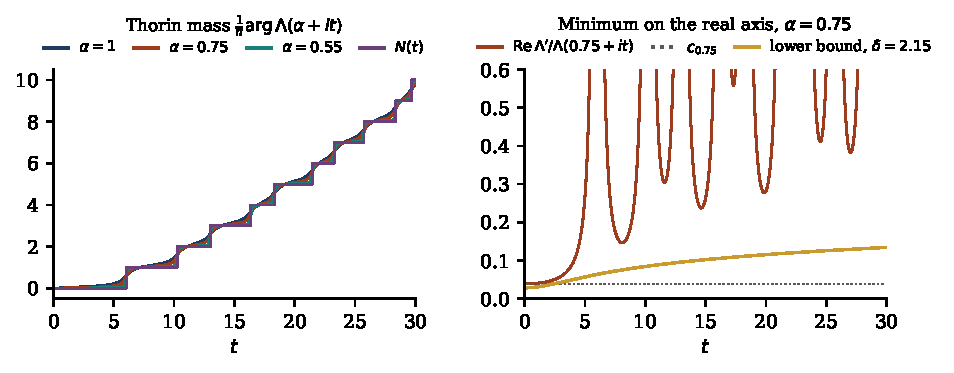
\includegraphics[width=\textwidth]{figs/beta_argument.pdf}
\caption{Left: cumulative Thorin mass $\tau_\alpha((0,t^2])=\pi^{-1}\arg\Lambda(\alpha+it)$ for $\alpha=1,\,0.75,\,0.55$ against the zero counting function $N(t)$ of $\beta$. Right: $\operatorname{Re}\,\Lambda'/\Lambda(0.75+it)$, its value $c_{0.75}$ at $t=0$, and the bound of Corollary~\ref{beta:cor:lower} with $\delta=2.15$, which exceeds $c_{0.75}$ for $t>2.434$.}
\label{beta:fig:arg}
\end{figure}


\section{The centre}\label{beta:sec:centre}

An unconditional input at the centre would be a positive structure of the primal law that does not come from the zeros. One candidate is a scale mixture of $\Gamma(2)$ densities with positive mixing measure, which is infinitely divisible by Kristiansen's theorem \cite{kristiansen1994} (Steutel's conjecture). For $\beta$ neither the two sided nor the one sided form of this holds.

By Remark~\ref{rem:10dnotid}, whose argument is that of Roynette and Yor \cite{roynetteyor2005} for $\xi$, $X_\beta$ is not infinitely divisible: its characteristic function $\Lambda(\tfrac12+it)/\Lambda(\tfrac12)$ vanishes at $t=6.0209489$ (it is $+0.006077$ at $t=5.9$ and $-0.003508$ at $t=6.1$). Nor is $\Lambda(\tfrac12+w)/\Lambda(\tfrac12)$ a positive mixture $\int M(d\lambda)/(w+\lambda)^2$ of $\Gamma(2)$ transforms, since such a mixture decreases on $w>0$ while $\Lambda(\tfrac12+w)$ increases there.

For $\beta$ the one sided object is $\Phi_\beta1_{\{u>0\}}$, whose Laplace transform
\[
\int_0^\infty e^{-wu}\Phi_\beta(u)\,du=\frac12\int_1^\infty x^{(s-1)/2}\eta(ix)^3\,dx,\qquad s=\tfrac12-w,
\]
is an incomplete Mellin transform of $\eta^3$, the analogue of the piece from $x=1$ to $\infty$ in Riemann's theta function proof of the functional equation of $\zeta$ \cite{titchmarsh1986}. It is not a $\Gamma(2)$ mixture either.

\begin{proposition}\label{beta:prop:nocm}
Neither $\Phi_\beta(u)/u$ on $u>0$ nor $\eta(ix)^3$ on $x>0$ is completely monotone; in particular $\Phi_\beta1_{\{u>0\}}$ is not a positive mixture of $\Gamma(2)$ densities.
\end{proposition}

\begin{proof}
A completely monotone $g=\int e^{-\lambda u}M(d\lambda)$ with $M\ne0$ satisfies $g(u)\ge M([0,L])e^{-Lu}$ for any $L$ with $M([0,L])>0$, so it decays at most exponentially, whereas $\Phi_\beta(u)/u$ decays like $\exp(\tfrac32u-\tfrac\pi4e^{2u})$. By \eqref{beta:eq:jacobi} and uniqueness of the Laplace transform, the representing measure of $\eta(ix)^3$ has the signed weights $(-1)^n(2n+1)$ at $\pi(2n+1)^2/4$.
\end{proof}

The decay argument applies to every degree one kernel, since all decay like $\exp(-ce^{2u})$: no P\'olya kernel of a degree one $L$ function, Riemann's kernel $\Phi$ of \eqref{eq:ch10polya} included, is of the form $\int u^{a-1}e^{-\lambda u}M(d\lambda)$ on a half line with $M\ge0$ and $a>0$.

The positivity sits in the reciprocal of the product: with $q=e^{-2\pi x}$ and $\sigma_{-1}(N)=\sum_{d\mid N}d^{-1}$,
\begin{equation}\label{beta:eq:recipprod}
\frac{e^{-\pi x/4}}{\eta(ix)^3}=\prod_{m\ge1}(1-q^m)^{-3}
=\exp\Bigl(3\sum_{N\ge1}\sigma_{-1}(N)\,e^{-2\pi Nx}\Bigr)
\end{equation}
is the exponential of a completely monotone function, hence completely monotone. As in Thorin's theory, the representing measure of $\eta(ix)^3$ is signed while the reciprocal of its product part is the exponential of a positive mixture.


\section{The Dedekind eta function and \texorpdfstring{$\chi_{12}$}{chi 12}}\label{beta:sec:eta}

Euler's pentagonal identity gives $\eta(ix)=\sum_{n\ge1}\chi_{12}(n)e^{-\pi n^2x/12}$, where $\chi_{12}$ is the real even primitive character modulo $12$ with $\chi_{12}(\pm1)=1$ and $\chi_{12}(\pm5)=-1$. As in Section~\ref{beta:sec:primal},
\[
\Lambda_{12}(s):=\Bigl(\frac{12}{\pi}\Bigr)^{s/2}\Gamma\Bigl(\frac s2\Bigr)L(s,\chi_{12})
=\int_0^\infty x^{s/2-1}\eta(ix)\,dx,
\]
so $\Lambda_{12}(\tfrac12+w)=2\int_{\R}e^{wu}\Phi_{12}(u)\,du$ with the even, strictly positive kernel $\Phi_{12}(u)=e^{u/2}\eta(ie^{2u})$, and $\Lambda_{12}(s)=\Lambda_{12}(1-s)$. The L\'evy measure for $\alpha>1$ is $dx/(1-e^{-2x})+\sum_{n\ge2}\chi_{12}(n)\Lambda(n)\delta_{\log n}$, again with positive archimedean and signed prime parts, and with $K=\mathbb Q(\sqrt3)$ one has $\zeta_K=\zeta\cdot L(s,\chi_{12})$.

\begin{theorem}[Real characters; after \cite{polson2018vdp}, Theorem~30 and Remark~32]\label{beta:thm:realchar}
Let $\chi$ be a real primitive character with quadratic field $K$. Then $T^\chi_\alpha(y)=\operatorname{Re}(\Lambda_\chi'/\Lambda_\chi)(\alpha+i\sqrt y)/(2\pi\sqrt y)=T^K_\alpha(y)-T^\xi_\alpha(y)$; by Theorem~\ref{thm:10dshift} the reciprocal $\Lambda_\chi(\alpha)/\Lambda_\chi(\alpha+\sqrt v)$ is a GGC transform for $\alpha\ge1$, and GRH for $\chi$ is equivalent to $T^K_\alpha\ge T^\xi_\alpha$ for every $\alpha>\tfrac12$; and Theorems~\ref{beta:thm:local} and \ref{beta:thm:comp} hold for $\Lambda_\chi$, as does Theorem~\ref{beta:thm:realaxis} when the theta kernel of $\chi$ is positive.
\end{theorem}

\begin{proof}
With $d_K$ the discriminant, put
\begin{align*}
\xi_K(s)&=\tfrac12s(s-1)|d_K|^{s/2}(2\pi)^{-s}\Gamma(s)\zeta_K(s)&&\text{for imaginary $K$},\\
\xi_K(s)&=\tfrac12s(s-1)|d_K|^{s/2}\pi^{-s}\Gamma(\tfrac s2)^2\zeta_K(s)&&\text{for real $K$};
\end{align*}
for $K=\mathbb Q(i)$ the first agrees with the definition above, since $4^{s/2}(2\pi)^{-s}=\pi^{-s}$. Then $\xi_K=c\,\xi\,\Lambda_\chi$ for a constant $c$ (by the duplication formula for imaginary $K$, directly for real $K$); the factor $|d_K|^{s/2}$ is essential, since without it the ratio acquires a factor $e^{ks}$ that shifts $\operatorname{Re}\,\xi_K'/\xi_K$ by a constant. The proofs above then apply to logarithmic derivatives.
\end{proof}

For $\chi_{12}$, $L(\sigma,\chi_{12})$ is $0.125$, $0.334$, $0.499$, $0.625$, $0.721$ at $\sigma=0.1$, $0.3$, $0.5$, $0.7$, $0.9$; the first ordinates are $3.8046$, $6.6922$, $8.8906$, $11.1884$; $V_{12}=0.33292$; the termwise threshold $\alpha_c(\chi_{12})=1.8349$ is the root of
\[
\tfrac12\log\tfrac{12}\pi+\tfrac12\psi(\tfrac\alpha2)=-\frac{\zeta'}\zeta(\alpha)-\frac{\log2}{2^\alpha-1}-\frac{\log3}{3^\alpha-1};
\]
and over $t\in[0,30]$ the minimum of $\operatorname{Re}\,\Lambda_{12}'/\Lambda_{12}(\alpha+it)$ is $c_\alpha$, equal to $0.16508$, $0.08306$, $0.03328$ at $\alpha=1,\,0.75,\,0.6$. The smaller threshold reflects the larger conductor term $\tfrac12\log\frac{12}{\pi}$ and the removal of the primes $2$ and $3$.

\subsection{Open problems}

\begin{problem}[A coupling below $\alpha=1$]\label{op:betacoupling}
Construct the coupling $H^K_\alpha\overset{d}{=}H^\xi_\alpha+H^\beta_\alpha$ of Theorem~\ref{beta:thm:dom} from the Gaussian primes in a form that could survive below $\alpha=1$. By Proposition~\ref{beta:prop:kron} it must use the phases $\chi_{-4}(p)p^{-it}$, not only the sizes of the atoms. A first computation is the smallest margin of $\operatorname{Re}\,\xi_K'/\xi_K-\operatorname{Re}\,\xi'/\xi$ on lines $\tfrac12<\alpha<1$.
\end{problem}

\begin{problem}[Negative windows]\label{op:betawindows}
Find a lower bound for the decrease of $\arg\Lambda(\alpha+it)$ across the window of Theorem~\ref{beta:thm:local} caused by a pair $\tfrac12\pm B+i\gamma$, in terms of $B$, $\alpha$ and the local density of zeros, that a mean value estimate for $\operatorname{Re}\,\Lambda'/\Lambda$ over intervals of length one could contradict.
\end{problem}

\begin{problem}[All lines to the right]\label{op:betalines}
Theorem~\ref{beta:thm:minall}(ii) places the minimum over $t$ of $\operatorname{Re}\,\Lambda'/\Lambda(\alpha+it)$ at $t=0$ for $\tfrac12<\alpha\le3.15$ and $|t|\le H_0-1.2071$. Extend it to every $\alpha>\tfrac12$ at these heights, either by optimising $\delta$ as a function of $\alpha$ or by a direct argument for large $\alpha$, where the prime part is small, and to every height for $\alpha\ge1$. Numerically the minimum over $t\in[0,40]$ is at $t=0$ for $\alpha=1.5,\,2,\,3,\,3.15$ and $5$. For $\xi$ the statement at every height is Lagarias's theorem under RH \cite{lagarias1999}, and unconditionally it is known for $\alpha\ge1$ \cite{garunkstis2002}; the arguments of Lagarias for $\alpha\ge10$, of Garunk\v{s}tis \cite{garunkstis2000,garunkstis2002} and of Broughan \cite{broughan2009} near $\alpha=1$ are natural routes for $\beta$.
\end{problem}

\begin{problem}[Positivity on the reciprocal side]\label{op:betarecip}
By \eqref{beta:eq:recipprod} and its analogue for $\eta$, the functions $e^{-\pi x/4}/\eta(ix)^3$ and $e^{-\pi x/12}/\eta(ix)$ are completely monotone, with representing measures at the points $2\pi n$, $n\ge0$, whose weights are the coefficients of $\prod_m(1-q^m)^{-3}$ and $\prod_m(1-q^m)^{-1}$. Decide whether this positivity passes, through incomplete Mellin transforms, to a positive representation on the reciprocal side of $\Lambda$ or of $\Lambda_{12}$.
\end{problem}


\section{Notes}

The Thorin framework of this chapter is that of Chapters~\ref{ch:10b} and \ref{ch:10d}. For real primitive characters, $\chi_{-4}$ among them, the closed form of the Thorin density, the GGC property for $\alpha>1$ and the equivalence of GRH with the GGC property at every $\alpha>\tfrac12$ are Theorem~30 and Remark~32 of \cite{polson2018vdp}, and Theorem~\ref{thm:10dshift} gives them, with $\alpha\ge1$, for every $L$ function of Chapter~\ref{ch:10b}; Theorems~\ref{beta:thm:thorin}, \ref{beta:thm:uncond} and \ref{beta:thm:grh}, and the corresponding parts of Theorems~\ref{beta:thm:dom} and \ref{beta:thm:realchar}, are their cases; the L\'evy form of Theorem~\ref{beta:thm:levy} is the computation of Section~\ref{sec:10daway} for an odd character. The Mellin form of Proposition~\ref{beta:prop:mellin} is the theta series proof of the functional equation for odd characters \cite{iwanieckowalski2004}, \cite[Section~8.1]{polson2018vdp} relates $\eta^3$ to $\beta$ through its Laplace transform, and Jacobi's identity for $\eta^3$ and Euler's pentagonal identity for $\eta$ are classical. Lemma~\ref{beta:lem:2sin2} is the signed form of Lemma~\ref{lem:10dsin2}, which is Lemma~14 of \cite{polson2018vdp} with a first step of Roynette and Yor \cite{roynetteyor2005}. The splitting $\zeta_K=\zeta\beta$ for $K=\mathbb Q(i)$ is classical, and the induction of the trivial character of $K$ to $1\boxplus\chi_{-4}$ is the simplest case of automorphic induction.

Proposition~\ref{beta:prop:kron} rests on Kronecker's theorem and the linear independence of the $\log p$, as in Proposition~\ref{prop:ch09notcf} and in the value distribution theory of Bohr and Jessen \cite{bohrjessen1930}. For $1<\alpha<\alpha_c\approx2.28$ the atoms of $\beta$ prove positivity only above the height $t_0(\alpha)$, and no bound that uses only their sizes does better; at $\alpha=1$ the nonvanishing of $\beta$ on $\operatorname{Re}s=1$ is what excludes atoms from the Thorin measure, as for $\xi$ in \cite[Remark~21]{polson2018vdp}.

For $\xi$ the minimum of $\operatorname{Re}\,\xi'/\xi$ on the line $\operatorname{Re}s=\alpha$ lies at $t=0$ unconditionally for $\alpha\ge10$ and, under RH, for every $\alpha>\tfrac12$, attained only at $t=0$ (Lagarias \cite{lagarias1999}, Theorems~1.2 and 1.3 and Section~3); Garunk\v{s}tis proved it unconditionally for $\alpha>4.5$ \cite{garunkstis2000} and for every $\alpha\ge1$ \cite{garunkstis2002}, both stated for the infimum, and Lemma~2.5 and Theorem~3.2 of Broughan \cite{broughan2009}, with the verification of RH to height $3\times10^{12}$ \cite{platttrudgian2021}, give the strict inequality for every $t\ne0$ when $\alpha\ge1.043$. The criterion that RH is equivalent to $\operatorname{Re}\,\xi'/\xi>0$ on $\operatorname{Re}s>\tfrac12$ is due to Hinkkanen \cite{hinkkanen1997} and Lagarias \cite{lagarias1999}. In the notation of \eqref{eq:10dU} the minimum at $t=0$ is the positivity of the Thorin density $U$ that remains when the $\tfrac12$ stable part is removed, which \cite[Remark~31]{polson2018vdp} shows can fail for $\Lambda(s,\chi)$ alone with $\chi$ a complex character modulo $5$. As far as we know the following are new in this form: Theorem~\ref{beta:thm:minall} for $\beta$ and its analogue for $\chi_{12}$; for $\xi$, the unconditional range $\tfrac12<\alpha<1$ below height $3\times10^{12}$; and the comparison lemma with its sharp constant $1+\sqrt2$. They are elementary consequences of the Hadamard product, the functional equation and the rigorous verifications of GRH for small conductors by Platt \cite{platt2016} and of RH by Platt and Trudgian \cite{platttrudgian2021}, and none of them proves a Riemann hypothesis. The grouping \eqref{beta:eq:pair} and its consequence, that $\operatorname{Re}\,\xi'/\xi(\sigma+it)$ can be negative only within distance $\tfrac12$ of the ordinate of a zero off the line, are due to Levinson and Montgomery \cite[Section~2]{levinsonmontgomery1974}, and Broughan \cite{broughan2009} uses the same grouping; Corollary~\ref{beta:cor:height} reads them as a localisation of negative Thorin density, a quantitative form of the negative dip noted after Theorem~\ref{thm:10dshift}.

For $\xi$, Theorem~\ref{beta:thm:arg} and Corollary~\ref{beta:cor:argmono} are Theorem~8.2 and part of Theorem~8.4 of \cite{polson2017}. That $X_\beta$ is not infinitely divisible is Remark~\ref{rem:10dnotid}, after Roynette and Yor \cite{roynetteyor2005}. The completely monotone reciprocal product \eqref{beta:eq:recipprod} is a candidate for an unconditional input at the centre on the reciprocal side (Open Problem~\ref{op:betarecip}), not a proof that one exists.

Theorem~\ref{beta:thm:realchar} lists what extends to every real primitive character; the minimum on the real axis, Theorem~\ref{beta:thm:minall}, is established here only for $\chi_{-4}$, $\chi_{12}$ and $\xi$, and Problem~\ref{cp:betareal} asks how far it extends. Problem~\ref{cp:betahecke} poses the same questions for the Hecke characters of $\mathbb Q(i)$, whose $L$ functions are those of $\mathrm{GL}(2)$ newforms with complex multiplication, to which Theorem~\ref{thm:10dshift} already applies.


\section{Exercises}

\begin{enumerate}
\item Prove $\operatorname{Re}\,w/(1-w)\le r/(1-r)$ for $|w|=r<1$, with equality only at $w=r$. Deduce $\operatorname{Re}\,\beta'/\beta(\alpha+it)\ge-S(\alpha)$ for $\alpha>1$, and check $S(2)=-\zeta'/\zeta(2)-\tfrac13\log2=0.339$.
\item Prove Lemma~\ref{beta:lem:comp} from the identity for $g'(w)$ in its proof. Show that $g'(0)>0$ exactly when $(\sqrt2-1)B<|u|<(1+\sqrt2)B$, that $g'(B^2-u^2)>0$ when $0<|u|<B$, and that $Q_B(a,0)/a$ has a pole at $a=B$; conclude that $a\mapsto Q_B(a,u)/a$ is nonincreasing on $a>0$ if and only if $|u|\ge(1+\sqrt2)B$.
\item Show that $x\mapsto a/(a^2+x^2)$ is strictly convex exactly for $|x|>a/\sqrt3$, that $Q_B(a,u)$ is odd in $a$, and that $\partial_u^2Q_B(a,u)=12a\,u^{-4}-40a(a^2+3B^2)u^{-6}+O(u^{-8})$. Where does the proof of Theorem~\ref{beta:thm:minall} use each fact?
\item From Stirling's formula derive the asymptotic of Theorem~\ref{beta:thm:arg} and the constant $\tfrac18$ of the zero counting formula after it. What is the constant for $L(s,\chi_{12})$, whose gamma factor is $\Gamma(\tfrac s2)$?
\item Show that a completely monotone $g=\int e^{-\lambda u}M(d\lambda)$ with $M\ne0$ satisfies $g(u)\ge M([0,L])e^{-Lu}$ whenever $M([0,L])>0$, and deduce that no P\'olya kernel of a degree one $L$ function is a positive mixture of $\Gamma(a)$ densities on a half line, for any $a>0$. Prove \eqref{beta:eq:recipprod}, compute the first five coefficients of $\prod_m(1-q^m)^{-3}$, and explain why the decay argument does not apply to $e^{-\pi x/4}/\eta(ix)^3$.
\item From Jacobi's identity \eqref{beta:eq:jacobi} show that the theta series of $\chi_{-4}$ is $\eta(ix)^3$, and deduce from $\eta(i/x)=\sqrt x\,\eta(ix)$ that $\Phi_\beta$ is even and positive. Do the same for $\Lambda_{12}$ and $\Phi_{12}$ with Euler's pentagonal identity.
\item For a real primitive character $\chi$ with quadratic field $K$ verify $\xi_K=c\,\xi\,\Lambda_\chi$, with $c=1$ for real $K$ and $c=1/(2\sqrt\pi)$ for imaginary $K$, and show that omitting the factor $|d_K|^{s/2}$ changes $\xi_K'/\xi_K$ by the constant $\tfrac12\log|d_K|$. Which statements of this chapter need the theta kernel of $\chi$ to be positive?
\item Show that $\Lambda(1)/\Lambda(1+\sqrt v)$ is a GGC transform, as the weak limit of the transforms at $\alpha\downarrow1$, without using the nonvanishing of $\beta$ on $\operatorname{Re}s=1$, and that a zero of $\beta$ at $1+i\gamma$ would give the Thorin measure at $\alpha=1$ an atom at $\gamma^2$.
\end{enumerate}


\section{Open computational problems}

Each problem can be attacked numerically first, with the closed form \eqref{beta:eq:Tclosed}, the argument form of Theorem~\ref{beta:thm:arg} and the comparison bound of Corollary~\ref{beta:cor:lower}; a sign found numerically is proved only by a computation with error control.

\begin{compproblem}[Minimum on the real axis for real characters]\label{cp:betareal}
Objective: for every real primitive character $\chi$ of conductor at most $10^3$, compute $V_\chi=(\log\Lambda_\chi)''(\tfrac12)$, the termwise threshold $\alpha_c(\chi)$ (for $\chi_{-4}$ and $\chi_{12}$ it is $2.2823$ and $1.8349$) with the heights $t_0(\alpha)$ of Proposition~\ref{beta:prop:kron}, the comparison height $t_1(\chi)$ of Theorem~\ref{beta:thm:minall} for the best $\delta$, and the lowest ordinate $\gamma_1(\chi)$, and record whether the theta kernel of $\chi$ is positive, which Theorem~\ref{beta:thm:realaxis} needs. List the characters with $t_1(\chi)+(\tfrac12+\delta)/\sqrt3\ge\gamma_1(\chi)$, for which the convexity step in the proof of part (ii) fails near the real axis; $\chi_{-163}$ is one, since its lowest ordinate is $0.2029<1/(2\sqrt3)$. Then test whether the minimum over $t$ of $\operatorname{Re}\,\Lambda_\chi'/\Lambda_\chi(\alpha+it)$ is attained at $t=0$ on every line $\tfrac12<\alpha\le10$. Objects and scale: the real primitive characters of conductor at most $10^3$, about six hundred; $\alpha$ on a grid of step $0.01$; $|t|\le100$. Route: PARI/GP (\texttt{lfuninit}, \texttt{lfunlambda}, \texttt{lfunzeros}) for $\Lambda_\chi$, its logarithmic derivative and its zeros, with the number of zeros checked by the argument principle; $\alpha_c(\chi)$ by root finding as in Section~\ref{beta:sec:eta}; ball arithmetic to prove the signs near the minima and for the characters near the failure boundary. Deliverable: a table by conductor and parity of $V_\chi$, $\alpha_c(\chi)$, $t_1(\chi)$, $\gamma_1(\chi)$, the sign of the kernel and the smallest margin over $t$ on each line; the exceptional characters, with a separate argument for part (ii) where one can be found; and fits of $V_\chi$, $\gamma_1(\chi)$ and $\alpha_c(\chi)$ against $\log q$. Why it matters: it shows how far Theorem~\ref{beta:thm:minall}, the analogue for $\beta$ of Lagarias's theorem \cite{lagarias1999}, reaches among real characters as the conductor grows and the lowest zero comes down, on average, towards the real axis; only the signs proved in ball arithmetic are verified.
\end{compproblem}

\begin{compproblem}[Hecke characters of the Gaussian field]\label{cp:betahecke}
Objective: for the Hecke characters \cite{hecke1918} $\lambda_k((a))=(a/|a|)^{4k}$ of $\mathbb Q(i)$, whose $L$ functions are those of the newforms with complex multiplication of weight $4k+1$ and level $4$, compute on lines $\alpha>\tfrac12$ the Thorin density of Theorem~\ref{thm:10dshift}, the termwise threshold $\alpha_c(\lambda_k)$ and the analogue of Proposition~\ref{beta:prop:kron}, the constants $V$ and $t_1$ and the first ordinate, and test the minimum on the real axis of Theorem~\ref{beta:thm:minall}, after checking the root number and the sign of the P\'olya kernel. Objects and scale: $k=1,\dots,5$, weights $5$ to $21$; ordinates to height $10^3$. Route: PARI/GP \texttt{mfinit} and \texttt{lfuncreate} for the newforms, or \texttt{gcharinit} for the characters, with \texttt{lfunzeros}; archimedean factor $\Gamma_{\mathbb C}(s+2k)$ in the unitary normalisation; atoms $2\cos(4km\theta_p)\log p$ at $p^m$ for split $p=\pi\bar\pi$ with $\theta_p=\arg\pi$, $2\log p$ at the even powers of inert $p$, and $(-1)^{km}\log2$ at $2^m$; ball arithmetic near the minima. Deliverable: for each $k$ the threshold, $V$, $t_1$, the first ordinate and the minimum of $\operatorname{Re}\,\Lambda'/\Lambda(\alpha+it)-c_\alpha$ for $\alpha\in\{0.6,0.75,1\}$ over the scanned range, with the lines on which the minimum leaves the real axis, compared with the real characters of Problem~\ref{cp:betareal}. Why it matters: the atoms are cosines of the angles of Gaussian primes rather than signs, so Kronecker's theorem acts on angles, and the problem tests whether the minimum on the real axis is special to Dirichlet characters.
\end{compproblem}

\begin{compproblem}[Synthetic off line zeros]\label{cp:betasynthetic}
Objective: insert a hypothetical pair $\tfrac12\pm B+i\gamma$, with its conjugates, into the true zeros of $\beta$ and measure (a) the decrease of $\arg\Lambda(\alpha+it)$ across the window of Theorem~\ref{beta:thm:local}; (b) the distance from the off line ordinate beyond which complete monotonicity in the width survives: under GRH, $(\alpha-\tfrac12)^{-1}\operatorname{Re}\,\Lambda'/\Lambda(\alpha+it)=\sum_{\gamma'}1/(w+(t-\gamma')^2)$ over the true ordinates $\gamma'$, with $w=(\alpha-\tfrac12)^2$, is a Stieltjes function of $w$ with representing function $\rho_t(x)=\sum_{\gamma'}e^{-x(t-\gamma')^2}$, while the pair adds $2e^{-cx}\cos\kappa x$ with $u=t-\gamma$, $c=u^2-B^2$ and $\kappa=2|u|B$, which changes sign, so the distance is the analogue of the constant $1+\sqrt2$ of Lemma~\ref{beta:lem:comp}; and (c) the depth of the negative lobe of the signed density $u_\varepsilon$ of Proposition~\ref{prop:scholzelobe} (whose $A$ and $B$ are $\gamma^2-B^2$ and $2\gamma B$ in the notation here), and whether the neighbouring zeros mask it. Objects and scale: $L(s,\chi_{-4})$, its zeros to height $10^3$, $B$ from $10^{-3}$ to $0.4$, ten values of $\gamma$, lines $\tfrac12<\alpha\le1$. Route: the true $\Lambda$ from PARI/GP \texttt{lfunlambda} times the Hadamard factors of the synthetic zeros; the closed forms of Theorem~\ref{beta:thm:arg} and Lemma~\ref{beta:lem:comp}; $\rho_t(x)$ on a logarithmic grid $10^{-4}\le x\le10^4$, with the tail of the zero sum bounded through the zero counting formula; ball arithmetic wherever a sign is claimed. Deliverable: the three quantities as functions of $B$, $\alpha$ (or $\varepsilon$) and the local density of zeros, and the smallest $B$ detected at each $\varepsilon$. Why it matters: it measures how visible a zero off the line is in the Thorin measure, in its argument and in the signed densities of Chapter~\ref{ch:scholze}, which is what Open Problems~\ref{op:betawindows} and \ref{op:scholzelobe} ask to turn into bounds; an experiment with synthetic zeros proves nothing about the true ones.
\end{compproblem}
